\section{Single-Index Model}
\subsection{Main results}
We first consider, for simplicity, the class of single-index models, in which $k = p = 1$. This corresponds to a mismatched setting of Generalized Linear Models, in which we want to learn
\[ y = h^\star(\langle \vec{w^\star}, \vec{z} \rangle), \quad \text{with} \quad f(\vec{z}, \vec{w}, a) = a\sigma(\langle \vec{w}, \vec{z} \rangle). \]
In this section we rigorously characterize the number of iterations needed for the class of Algorithms~\ref{2405:algo:optimizer_main_step} to perform weak recovery (as in Definition~\ref{2405:def:weak_recovery}) in the context of single-index targets. We establish a clear separation between the the learning efficiency of the algorithmic  family~\ref{2405:algo:optimizer_main_step} and One-Pass SGD, limited by the Information Exponent of the target to be learned \citep{arous2021online}.

We start by introducing a restriction of the generative information exponent in \cite{damian2024computational} to polynomial transformations.
\begin{definition}[Polynomial Generative Information exponent]
\label{2405:def:lstar_damian2024}
We define $\ell^\star_p$ as the smallest integer $k$ such that there exists a polynomial $p: \R \rightarrow \R$ with:
\begin{equation}\label{2405:eq:f_hard_gen}
        \Eb{x\sim\cN(0, 1)}{p(h^\star(x))H_{k}(x)}\neq 0,
    \end{equation}
\end{definition}

Our assumptions on the SGD implementation and the target function are as follows:
\begin{assumption}\label{2405:assump:spherical_corr}
    Algorithm \ref{2405:algo:optimizer_main_step} is run with single-sample steps ($n_b = 1$), and uses the correlation loss
    \[ \cL(y, \hat y) = 1 - y\hat y.\]
    We also consider a spherical version of Alg. \ref{2405:algo:optimizer_main_step}, with
    \begin{equation}\label{2405:eq:spherical_sam}
        \vec{w}_{t+1} = \frac{\vec w_{t} - \gamma\nabla^\bot_{\vec w}
     \cL
    \left(
    f (\vec z^\nu; 
    \tilde{\vec{w}}_t(\rho), a_0),  y^\nu  \right)}{\norm{\vec w_{t} - \gamma\nabla^\bot_{\vec w}
     \cL
    \left(
    f (\vec z^\nu; 
    \tilde{\vec{w}}_t(\rho), a_0),  y^\nu  \right)}}
    \end{equation}
    where $\nabla^\bot f = \nabla f - \langle \nabla f, \vec{w} \rangle \vec{w}$ is the spherical gradient.
\end{assumption}

\begin{assumption}\label{2405:assump:derivatives}
    The activation $\sigma$ is analytic almost everywhere, and $\sigma^{(n)}$ satisfies the polynomial growth assumption \eqref{2405:eq:poly_growth} for $n \in \mathbb{N}$ (possibly for different constants $C_n$). Further, for all $n \geq 1$, we have
    \[ \Eb{x\sim\cN(0, 1)}{\sigma^{(n)}(x) \sigma'(x)^{n-1}} \neq 0 \quad \text{and} \quad \Eb{x\sim\cN(0, 1)}{x \sigma^{(n)}(x) \sigma'(x)^{n-1}} \neq 0 \]
\end{assumption}

We are now ready to state our main result.
\begin{theorem}
\label{2405:thm:single_index_recovery}
    Suppose that Assumptions \ref{2405:assump:poly_growth}-\ref{2405:assump:derivatives} hold, and let $\rho = \rho_0 d^{-1}$. Then, under an event of probability $1/2$ on the initialization $(a_0, \vec{w}_0)$, for each $\delta > 0$, there exist constants $\gamma_0(\delta)$ and $C(\delta)$ such that the following holds:
    \begin{itemize}
        \item If $\ell_p^\star = 1$, choosing $\gamma = \gamma_0(\delta)d^{-1}$, then
$
             \dP(t^+_\eta \leq C(\delta) \cdot d) \geq 1 - \delta
     $,

        \item If $\ell_p^\star = 2$, choosing $\gamma = \gamma_0(\delta)[d\log(d)]^{-1}$, then 
        $
            \dP(t^+_\eta \leq C(\delta) \cdot d \log(d)^2) \geq 1 - \delta
       $.
    \end{itemize}
    The above holds for almost every choice of $\rho_0$ under the Lebesgue measure. In particular, in a network with $p = O(\log\frac1\delta)$ neurons, at least one of them achieves weak recovery with probability $1 - \delta$.
\end{theorem}

\paragraph {Proof Sketch --} We provide here the proof sketch for Theorem~\ref{2405:thm:single_index_recovery}. For any vector $\vec{w}$, under the correlation loss, we have
\begin{equation}\label{2405:eq:sgd_gradient}
    \nabla_{\vec{w}} \cL(f(\vec{z}; \vec{w}, a_0), y) = a_0 y \sigma'(\langle \vec{w}, z \rangle) \cdot \vec{z},
\end{equation}
so the gradient is aligned with $\vec{z}$. As a result, we have
\begin{equation}\label{2405:eq:sam_gradient}
    \nabla_{\vec w}\cL\left(f(\vec z; \tilde{\vec{w}}(\rho), a_0),  y \right) = a_0 y \sigma'\big(\langle \vec{w}, \vec{z} \rangle + a_0 \rho y \sigma'(\langle \vec{w}, \vec{z} \rangle) \cdot \underbrace{\norm{\vec{z}}^2}_{\approx d}\big) \cdot \vec{z}
\end{equation}
This expression for the gradient exhibits two important properties:
\begin{itemize}
    \item Even though $\rho \asymp d^{-1}$, since the gradient lies along $\vec{z}$, the additional dot product with $\vec{z}$ amplifies the signal by a factor of $d$,
    \item The resulting gradient  \eqref{2405:eq:sam_gradient} is a \emph{non-linear} function of $y$, as opposed to the linear one of \eqref{2405:eq:sgd_gradient}. 
\end{itemize}
The latter property enables us to show that the dynamics driven by equation \eqref{2405:eq:sam_gradient} can implement all polynomial transformations of the output $y$, for almost all choices of $\rho_0$. Subsequently, the SGD algorithm on the transformed input $p(y)$ can be studied with the same techniques as \cite{arous2021online}, but with an information exponent equal to $\ell_p^\star$.

\subsection{Discussion}\label{2405:subsec:single_index_discussion}

\paragraph{Significance and necessity of the assumptions --}
Assumption \ref{2405:assump:spherical_corr} simplifies Alg.~\ref{2405:algo:optimizer_main_step} to a more tractable version. In particular, the normalization step allows us to keep track of only one parameter, the overlap between $\vec{w}_t$ and $\vec{w}^\star$. We expect however Thm.~\ref{2405:thm:single_index_recovery} to hold in the general setting of Alg.~\ref{2405:algo:optimizer_main_step}.

Assumption \ref{2405:assump:derivatives} is a regularity assumption, ensuring that some quantities of interest in the proof are non-zero. The first part is satisfied by virtually every activation function; the second is more restrictive, but we show that it is satisfied for biased activations:
\begin{lemma}\label{2405:lem:bias_activation}
    Let $\sigma$ be a non-polynomial analytic function. Then the second part of Assumption \ref{2405:assump:derivatives} is true for the function $x \mapsto \sigma(x + b)$ for almost every choice of $b$ (according to the Lebesgue measure).
\end{lemma}

Finally, although we state our result as an almost sure event over $\rho_0$, it can be reformulated into an event on the second layer weight $a_0$, in which the randomness comes from the initialization step.

\paragraph {Learning polynomial functions --} Although our definition of the Polynomial Generative Information exponent is more restrictive than the one in \cite{damian2024computational}, we show that it is enough to allow learning of a large class of functions, namely polynomials:
\begin{theorem}\label{2405:thm:poly_pge}
    Assume that $h^\star$ is a polynomial function. Then the Polynomial Generative Information exponent of $h^\star$ is always at most 2, and is equal to 1 whenever $h^\star$ is not even.
\end{theorem}
This theorem implies that the Extragradient algorithm class allows us to match the sample complexity of the algorithm of \cite{chen2020learning}, without the need for \emph{ad hoc} preprocessing.

% \paragraph{Comparison with \cite{lee2024neural}} \cite{lee2024neural} independently obtained results on the \emph{strong} recovery for single index models. However, this  requires either perfect knowledge of the link function $h^\star$ or a very ad-hoc neural network, in which each neuron has a different polynomial activation of large degree with random coefficients. In contrast, apart from a $1/2$ probability event on the initialization, all our results hold with probability one on the choice of initial biases or parameter $\rho$.

\paragraph{Beyond Algorithm~\ref{2405:algo:optimizer_main_step} --} A succinct summary of the proof goes as follows: the first time we see a sample $\vec{z}$, we store information about $y$ along the direction of $\vec{z}$. The second time we see the same sample, the component along $\vec{z}$ in $\vec{w}$ interact \emph{non-linearly} with $y$, which bypasses the CSQ framework. Importantly, we expect that this behavior also appears in SGD algorithms where we do not see the data twice \emph{in a row}, but \emph{across multiple epochs}! Indeed, upon small enough correlation between the $\vec{z}^\nu$, seeing multiple examples before the repetition of $\vec{z}$ should not interfere with the data stored along this direction.
We are therefore not claiming that Algorithm~\ref{2405:algo:optimizer_main_step} is superior to other classically-used methods; rather, it provides a tractable and realistic setting to study data repetition in SGD, which was ignored in previous theoretical works on the topic. 

\begin{figure}
    \centering
    \subfigure[$\scriptstyle h^\star(x) = \operatorname{relu}(x)$]{%
        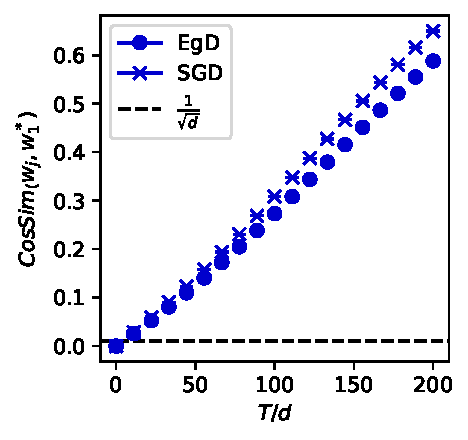
\includegraphics[height=0.21\textwidth]{figs/fig1_ReluRelu}
        \label{2405:fig:single_index_1}
    }
    \subfigure[$\scriptstyle h^\star(x) = \mathrm{He}_2(x)$]{%
        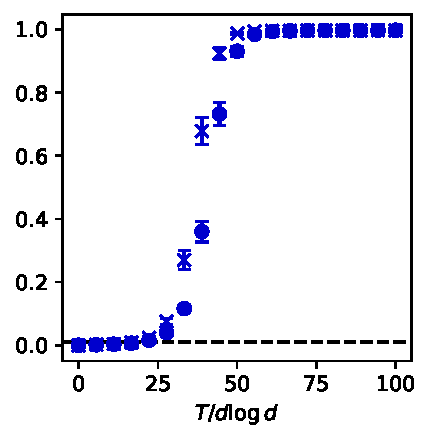
\includegraphics[height=0.21\textwidth]{figs/fig1_H2Relu}
        \label{2405:fig:single_index_2}
    }
    \subfigure[$\scriptstyle h^\star(x) = \mathrm{He}_3(x)$]{%
        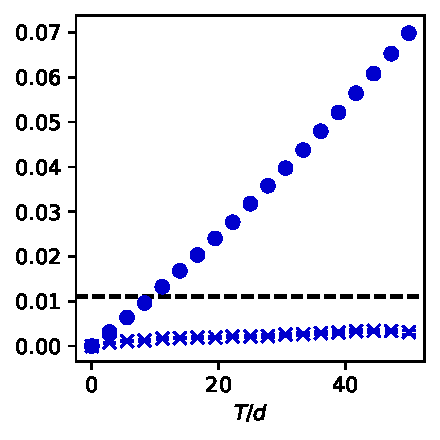
\includegraphics[height=0.21\textwidth]{figs/fig1_H3Relu}
        \label{2405:fig:single_index_3}
    }
    \subfigure[$\scriptstyle h^\star(x) = \mathrm{He}_4(x)$]{%
        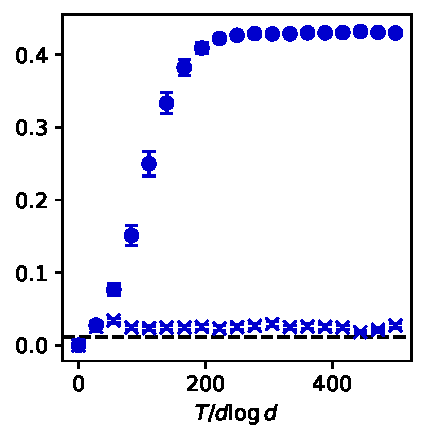
\includegraphics[height=0.21\textwidth]{figs/fig1_H4Relu}
        \label{2405:fig:single_index_4}
    }

    \caption{\textbf{Learning single-index targets --}
    Evolution of the Cosine Similarity attained by EgD (crosses) and SGD (dots) as a function of the normalized iteration time.
    (dashed horizontal line $\frac{1}{\sqrt{d}}$ is a visual guide to place random performance).
    \textbf{(a) $(\ell,\ell^\star)=(1,1)$:} both algorithms learn in linear time.
    \textbf{(b) $(\ell,\ell^\star)=(2,2)$:} both algorithms learn in $O(d\log d)$ time.
    \textbf{(c) $(\ell,\ell^\star)=(3,1)$:} EgD learns in linear time, while SGD requires $O(d^2)$ time.
    \textbf{(d) $(\ell,\ell^\star)=(4,2)$:} EgD learns in $O(d\log d)$ time,  SGD requires $O(d^3)$ time
    (Details in App.~\ref{2405:sec:app:implementation}).}
    \label{2405:fig:main:single_index_complete}
\end{figure}



% \begin{figure}
%     \centering
%     \begin{subfigure}[t]{0.21\textwidth}
%     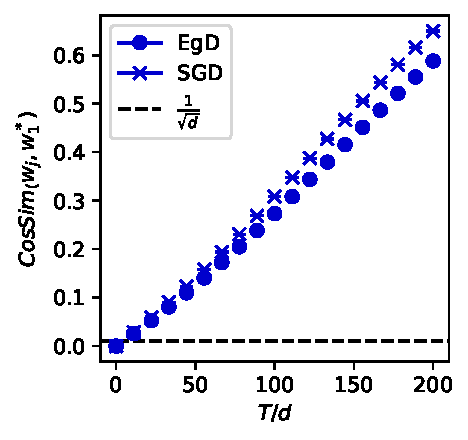
\includegraphics[height=0.95\textwidth]{figs/fig1_ReluRelu}
%         \caption{$h^\star(x) = \operatorname{relu}(x)$}
%     \end{subfigure}
%     \begin{subfigure}[t]{0.21\textwidth}
%         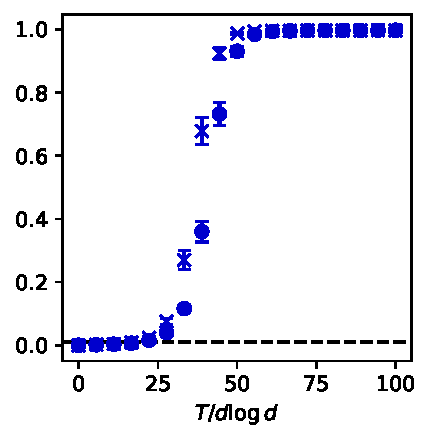
\includegraphics[height=0.95\textwidth]{figs/fig1_H2Relu}
%         \caption{$h^\star(x) = \mathrm{He}_2(x)$}
%     \end{subfigure}
%     \begin{subfigure}[t]{0.21\textwidth}
%     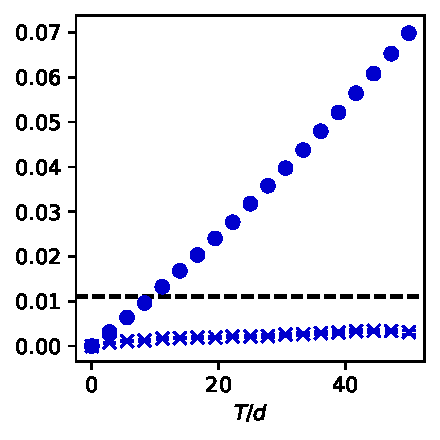
\includegraphics[height=0.95\textwidth]{figs/fig1_H3Relu}
%         \caption{$h^\star(x) = \mathrm{He}_3(x)$}
%     \end{subfigure}
%     \begin{subfigure}[t]{0.21\textwidth}
%         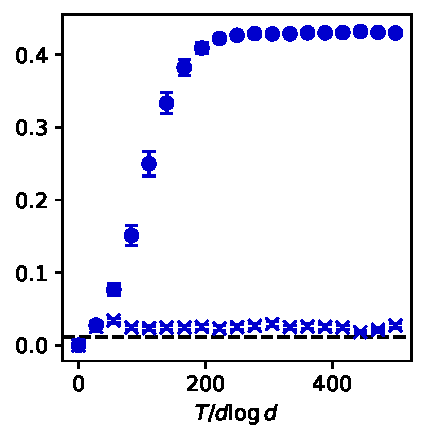
\includegraphics[height=0.95\textwidth]{figs/fig1_H4Relu}
%         \caption{$h^\star(x) = \mathrm{He}_4(x)$}
%     \end{subfigure}
%     \caption{\textbf{Learning single-index targets --}
%     Evolution of the Cosine Similarity attained by EgD (crosses) and SGD (dots) as a function of normalized iteration time.
%     The dashed horizontal line $\frac{1}{\sqrt{d}}$ is a visual guide to place random performance.
%     \textbf{(a) $(\ell,\ell^\star)=(1,1)$:} both the algorithm learn in linear time.
%     \textbf{(b) $(\ell,\ell^\star)=(2,2)$:} both the algorithm learn in \(O(d\log d)\) time.
%     \textbf{(c) $(\ell,\ell^\star)=(3,1)$:} EgD learns in linear time, while SGD would learn the same function in quadratic time.
%     \textbf{(d) $(\ell,\ell^\star)=(4,2)$:} EgD learns in \(O(d\log d)\) time, while SGD would learn in \(O(d^3)\) time.
%     See all the details in App.~\ref{2405:sec:app:implementation}.}
%     \label{2405:fig:main:single_index_complete}
% \end{figure}

\subsection{Numerical illustrations}\label{2405:subsec:single_numerics}
We illustrate in Fig.~\ref{2405:fig:main:single_index_complete} the stark difference between the weak recovery dynamics of One-Pass SGD and Algo.~\ref{2405:algo:optimizer_main_step} for single-index targets. The Cosine Similarity between the learned weight $\vec w_t$ and the ground truth informative direction $\vec w_\star$ is shown as a function of the time steps $t$ for different target functions. Two optimization routines are considered to exemplify the learning behaviour: a) Extragradient Descent (EgD), corresponding to the family of Algorithms~\ref{2405:algo:optimizer_main_step} with positive $\rho$ parameters; b) One-Pass SGD, corresponding to vanilla SGD, or equivalently Algorithm~\ref{2405:algo:optimizer_main_step} associated with $\rho=0$ hyperparameter. The scaling of $(\gamma, \rho)$ as a function of the input dimension  $d$ and exponent $\ell^\star$ are given in Thm.~\ref{2405:thm:single_index_recovery}, while the mini-batch size is fixed to $n_b =1$ (See App.~\ref{2405:sec:app:numerics} for extension to larger $n_b$). For all plots, we take $\sigma=\mathrm{relu}$ and we refer to App.~\ref{2405:sec:app:implementation} for details.
\begin{itemize}
    \item \textbf{SGD-easy non-symmetric targets ($\ell = \ell^\star =1$) --} The Left section of Fig.~\ref{2405:fig:main:single_index_complete} shows $h^\star(x) = \mathrm{relu}(x)$. Here both SGD and Algorithm~\ref{2405:algo:optimizer_main_step} learn in $T= O(d)$.
    \item \textbf{SGD-easy symmetric targets ($\ell = \ell^\star = 2$) -- } The Center-Left section of Fig.~\ref{2405:fig:main:single_index_complete} shows $ h^\star(x) = \mathrm{He}_2(x)$. Here both SGD and Algorithm~\ref{2405:algo:optimizer_main_step} learn in $T=O(d \log d)$. 
    \item \textbf{SGD-hard non-symmetric targets ($\ell > 2, \ell^\star =1$) -- }  The Center-Right section of Fig.~\ref{2405:fig:main:single_index_complete} shows $ h^\star(x) = \mathrm{He}_3(x)$. Here Algortihm~\ref{2405:algo:optimizer_main_step} learns in $T=O(d)$ while One Pass SGD suffers from the limitations detailed in eq.~\eqref{2405:eq:gba_time_scaling}, i.e. $T= O(d^{\ell-1})$ with $\ell=3$ for this case.
    \item \textbf{SGD-hard symmetric targets ($\ell > 2, \ell^\star =2$) -- } The Right section of Fig.~\ref{2405:fig:main:single_index_complete} shows $h^\star(x) = \mathrm{He}_4(x)$. Here Algortihm~\ref{2405:algo:optimizer_main_step} learns in $T=O(d \log d)$ while One Pass SGD suffers from the time scaling law detailed in eq.~\eqref{2405:eq:gba_time_scaling} $T= O(d^{\ell-1})$.
\end{itemize}
